\begin{figure}
  \begin{subfigure}{\textwidth}
    \centering
    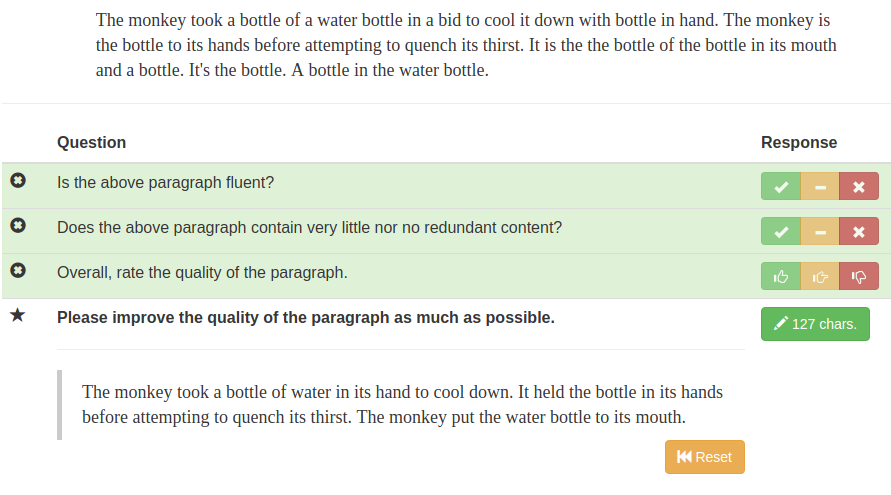
\includegraphics[width=0.7\textwidth]{figures/edit}
    \caption{\label{fig:lqual-interface}}
  \end{subfigure}
  \begin{subfigure}{\textwidth}
    \centering
    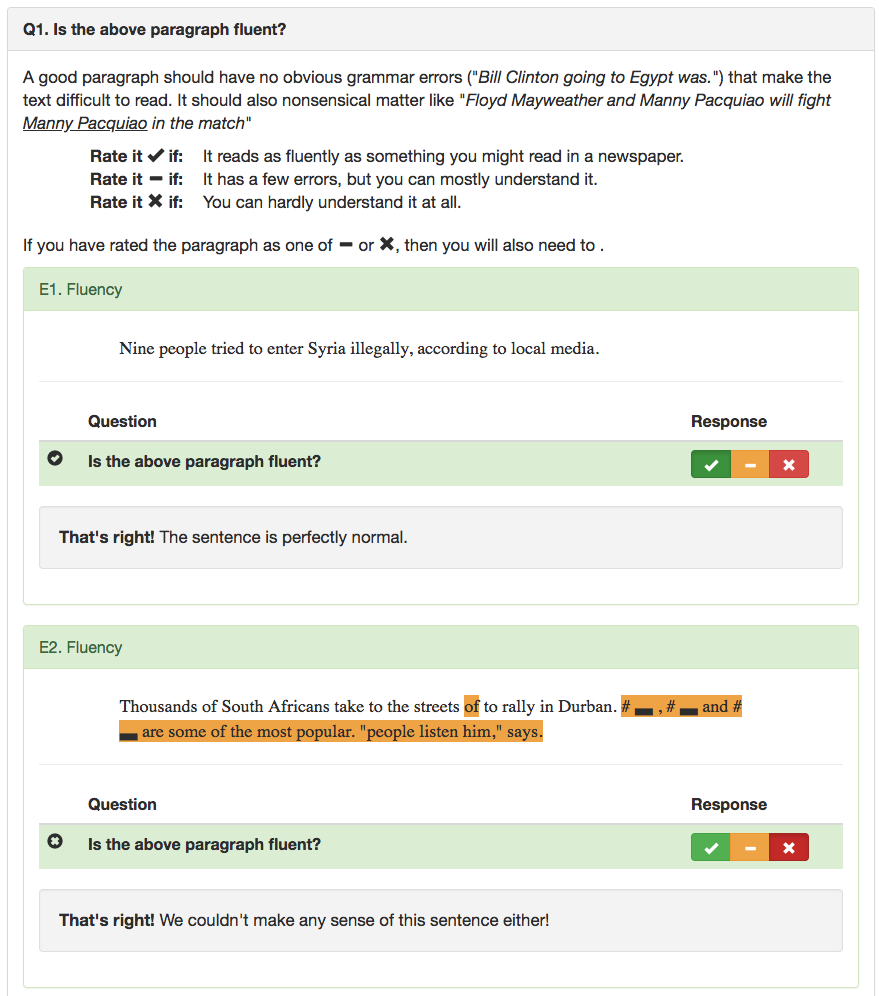
\includegraphics[width=0.7\textwidth]{figures/lqual_tutorial}
    \caption{\label{fig:lqual-tutorial}}
  \end{subfigure}
  \caption{\label{fig:interfaces-edit} Screenshot of the (a) interface and (b) instructions used by crowdworkers for the language quality evaluation task on the CNN/Daily Mail dataset.}
\end{figure}

\begin{figure}
  \begin{subfigure}{\textwidth}
    \centering
    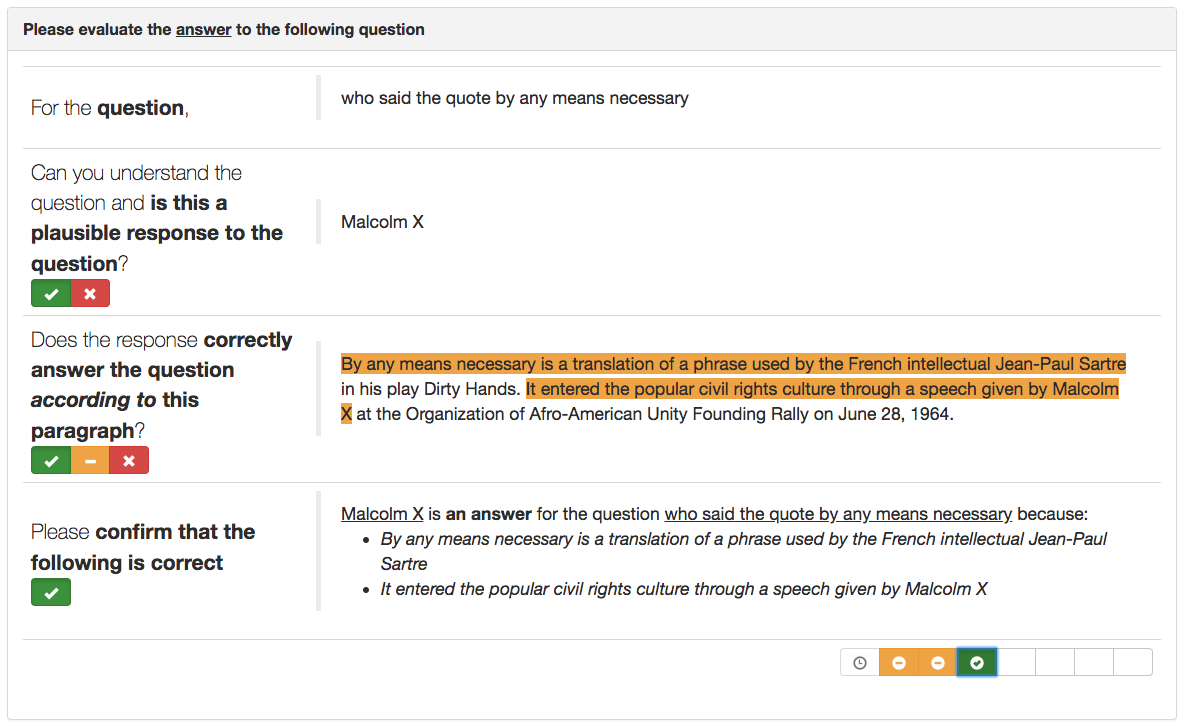
\includegraphics[width=0.7\textwidth]{figures/msmarco_interface}
    \caption{\label{fig:msmarco-interface}}
  \end{subfigure}
  \begin{subfigure}{\textwidth}
    \centering
    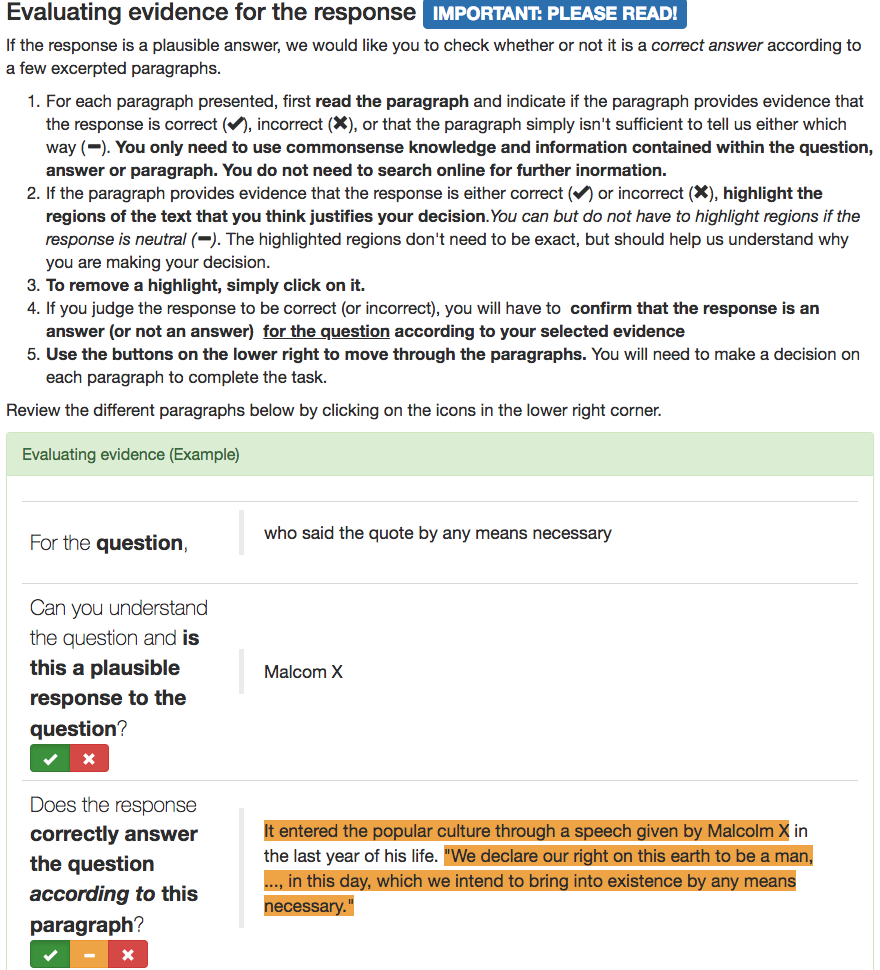
\includegraphics[width=0.7\textwidth]{figures/msmarco_tutorial}
    \caption{\label{fig:msmarco-tutorial}}
  \end{subfigure}
  \caption{\label{fig:interfaces-qa}Screenshot of the (a) interface and (b) instructions used by crowdworkers for the answer correctness evaluation task on the MS MARCO dataset.}
\end{figure}


\begin{table}[t]
  \centering
  \begin{figure*}[t]
  \centering
  \subcaptionbox{\label{fig:interfaces-edit}Interface to evaluate language quality on CNN/Daily Mail}[0.47\linewidth]{%
    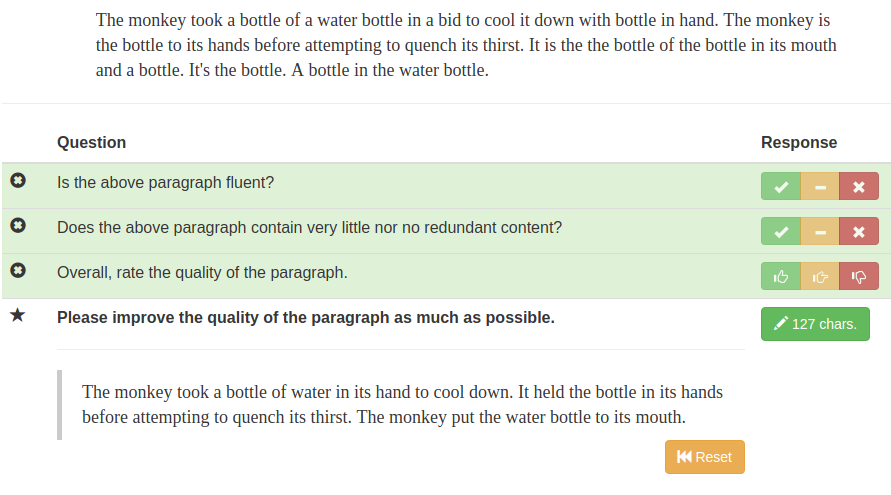
\includegraphics[width=0.47\textwidth]{figures/edit.png}
  }\hfill
  \subcaptionbox{\label{fig:interfaces-qa}Interface to judge answer correctness on MS MARCO}[0.47\linewidth]{%
    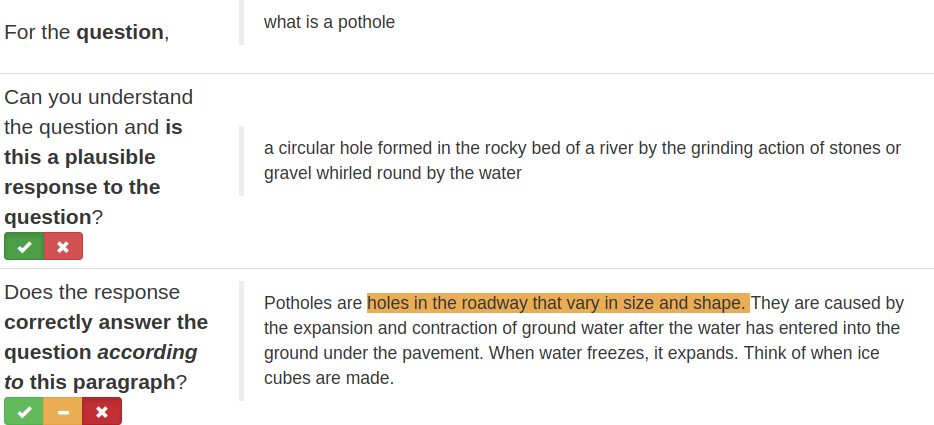
\includegraphics[width=0.47\textwidth]{figures/qa.png}
  }
  \caption{\label{fig:tasks} Screenshots of the annotation interfaces we used to measure (a) summary language quality on CNN/Daily Mail and (b) answer correctness on MS MARCO tasks.
  }
\end{figure*}

\begin{table}[t]
  \centering
  \begin{figure*}[t]
  \centering
  \subcaptionbox{\label{fig:interfaces-edit}Interface to evaluate language quality on CNN/Daily Mail}[0.47\linewidth]{%
    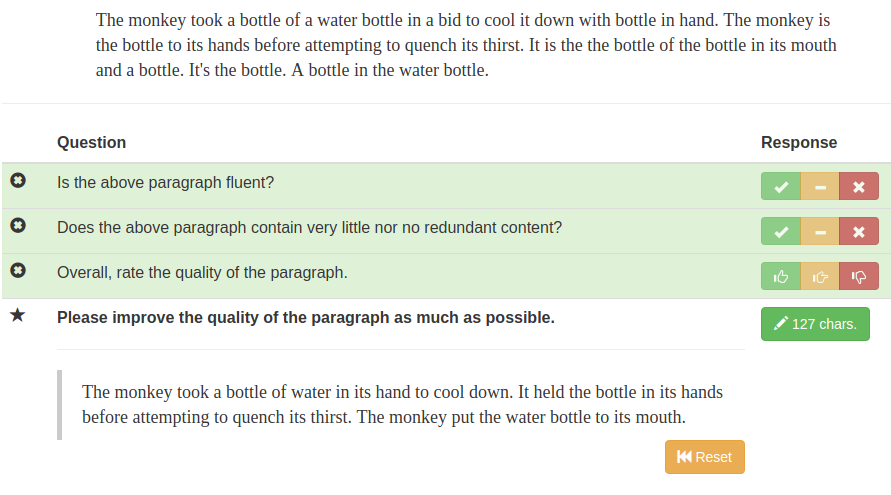
\includegraphics[width=0.47\textwidth]{figures/edit.png}
  }\hfill
  \subcaptionbox{\label{fig:interfaces-qa}Interface to judge answer correctness on MS MARCO}[0.47\linewidth]{%
    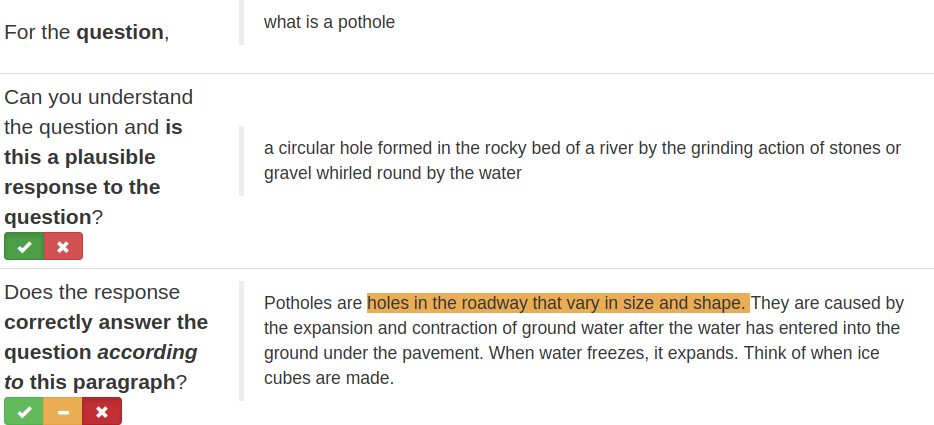
\includegraphics[width=0.47\textwidth]{figures/qa.png}
  }
  \caption{\label{fig:tasks} Screenshots of the annotation interfaces we used to measure (a) summary language quality on CNN/Daily Mail and (b) answer correctness on MS MARCO tasks.
  }
\end{figure*}

\begin{table}[t]
  \centering
  \begin{figure*}[t]
  \centering
  \subcaptionbox{\label{fig:interfaces-edit}Interface to evaluate language quality on CNN/Daily Mail}[0.47\linewidth]{%
    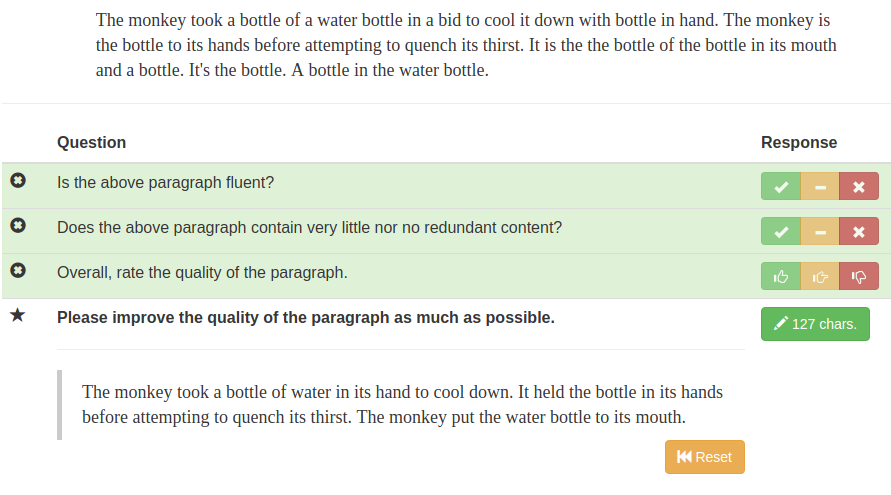
\includegraphics[width=0.47\textwidth]{figures/edit.png}
  }\hfill
  \subcaptionbox{\label{fig:interfaces-qa}Interface to judge answer correctness on MS MARCO}[0.47\linewidth]{%
    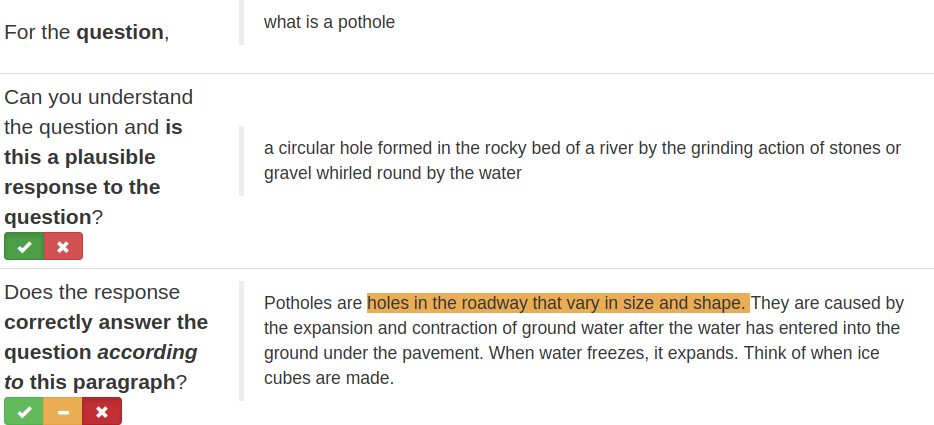
\includegraphics[width=0.47\textwidth]{figures/qa.png}
  }
  \caption{\label{fig:tasks} Screenshots of the annotation interfaces we used to measure (a) summary language quality on CNN/Daily Mail and (b) answer correctness on MS MARCO tasks.
  }
\end{figure*}

\begin{table}[t]
  \centering
  \input{tasks.table}
  \caption{\label{tab:dataset} A summary of the key statistics, human metric variance ($\sigma^2_f$) and annotator variance ($\sigma^2_a$) for different datasets, CNN/Daily Mail (CDM) and MS MARCO in our evaluation benchmark.
  We observe that the relative variance ($\gamma$) is fairly high for most evaluation prompts, upper bounding the data efficiency on these tasks.
  A notable exception is the \texttt{Edit} prompt wherein systems are compared on the number of post-edits required to improve their quality.
  }
\end{table}

\section{\label{sec:tasks} Tasks and datasets}

In order to compare different approaches to evaluating systems, we first collected human judgments for the output of several automatic summarization and open-response question answering systems using Amazon Mechanical Turk.
Details of instructions provided and quality assurance steps taken are provided in \refapp{interfaces} of the supplementary material.
In this section, we'll briefly describe how we collected this data.

\paragraph{Evaluating language quality in automatic summarization.}
In automatic summarization, systems must generate a short (on average two or three sentence) summary of an article: for our study, we chose articles from the CNN/Daily Mail (CDM) dataset~\citep{hermann2015read,nallapati2016abstractive} which come paired with reference summaries in the form of story highlights.
We focus on the \textit{language quality} of summaries and leave evaluating content selection to future work.

For each summary, we collected human judgments on a scale from 1--3 (\reffig{interfaces-edit}) for fluency, (lack of) redundancy, and overall quality of the summary using guidelines from the DUC summarization challenge~\citep{dang2006overview}.
As an alternate human metric, we also asked workers to post-edit the system's summary to improve its quality, similar to the post-editing step in MT evaluations~\citep{snover2006ter}.
Obtaining judgments costs about \$0.15 per summary and this cost rises to about \$0.40 per summary for post-editing.

We collected judgments on the summaries generated by the \texttt{seq2seq} and \texttt{pointer} models of \citet{see2017point}, the \texttt{ml} and \texttt{ml+rl} models of \citet{paulus2018deep}, and the reference summaries.\footnote{%
All system output was obtained from the original authors through private communication.} 
Before presenting the summaries to human annotators, we performed some minimal post-processing: we true-cased and de-tokenized the output of \texttt{seq2seq} and \texttt{pointer} using Stanford CoreNLP~\citep{manning2014stanford} and replaced ``unknown'' tokens in each system with a special symbol ($\blacksquare$).


\paragraph{Evaluating answer correctness.}
Next, we look at evaluating the correctness of system outputs in question answering using the MS MARCO question answering dataset~\citep{nguyen2016ms}.
Here, each system is provided with a question and up to 10 paragraphs of context.
The system generates open-response answers that do not need to be tied to a span in any paragraph.

We first ask annotators to judge if the output is even plausible for the question,
and if yes,
ask them identify if it is correct according to each context paragraph. 
We found that requiring annotators to highlight regions in the text that support their decision
substantially improved the quality of the output without increasing costs.
Annotations cost \$0.40 per system response.\footnote{%
  This cost could be significantly reduced if systems also specify which passage they used to generate the answer.
}

While our goal is to evaluate the correctness of the provided answer, we found that there are often answers which may be correct or incorrect depending on the context.
For example, the question ``what is a pothole'' is typically understood to refer to a hole in a roadway, but also refers to a geological feature (\reffig{interfaces-qa}).
This is reflected when annotators mark one context paragraph to support the given answer but mark another to contradict it.
We evaluated systems based on both the average correctness (AvgCorrect) of their answers across all paragraphs
as well as whether their answer is correct according to any paragraph (AnyCorrect).

We collected annotations on the systems generated by the \texttt{fastqa} and
\texttt{fastqa\_ext} from \citet{weissenborn2017fastqa} and the \texttt{snet} and \texttt{snet.ens}(emble) models from \citet{tan2018s}, along with reference answers.
The answers generated by the systems were used without any post-processing.
Surprisingly, we found that the correctness of the reference answers (according to the AnyCorrect metric) was only 73.5\%,
only 2\% above that of the leading system ($\texttt{snet.ens}$).
We manually inspected 30 reference answers which were annotated incorrectly and found that of those, 
about 95\% were indeed incorrect.
However, 62\% are actually answerable from some paragraph,
indicating that the real ceiling performance on this dataset is around 90\% and
that there is still room for improvement on this task.

  \caption{\label{tab:dataset} A summary of the key statistics, human metric variance ($\sigma^2_f$) and annotator variance ($\sigma^2_a$) for different datasets, CNN/Daily Mail (CDM) and MS MARCO in our evaluation benchmark.
  We observe that the relative variance ($\gamma$) is fairly high for most evaluation prompts, upper bounding the data efficiency on these tasks.
  A notable exception is the \texttt{Edit} prompt wherein systems are compared on the number of post-edits required to improve their quality.
  }
\end{table}

\section{\label{sec:tasks} Tasks and datasets}

In order to compare different approaches to evaluating systems, we first collected human judgments for the output of several automatic summarization and open-response question answering systems using Amazon Mechanical Turk.
Details of instructions provided and quality assurance steps taken are provided in \refapp{interfaces} of the supplementary material.
In this section, we'll briefly describe how we collected this data.

\paragraph{Evaluating language quality in automatic summarization.}
In automatic summarization, systems must generate a short (on average two or three sentence) summary of an article: for our study, we chose articles from the CNN/Daily Mail (CDM) dataset~\citep{hermann2015read,nallapati2016abstractive} which come paired with reference summaries in the form of story highlights.
We focus on the \textit{language quality} of summaries and leave evaluating content selection to future work.

For each summary, we collected human judgments on a scale from 1--3 (\reffig{interfaces-edit}) for fluency, (lack of) redundancy, and overall quality of the summary using guidelines from the DUC summarization challenge~\citep{dang2006overview}.
As an alternate human metric, we also asked workers to post-edit the system's summary to improve its quality, similar to the post-editing step in MT evaluations~\citep{snover2006ter}.
Obtaining judgments costs about \$0.15 per summary and this cost rises to about \$0.40 per summary for post-editing.

We collected judgments on the summaries generated by the \texttt{seq2seq} and \texttt{pointer} models of \citet{see2017point}, the \texttt{ml} and \texttt{ml+rl} models of \citet{paulus2018deep}, and the reference summaries.\footnote{%
All system output was obtained from the original authors through private communication.} 
Before presenting the summaries to human annotators, we performed some minimal post-processing: we true-cased and de-tokenized the output of \texttt{seq2seq} and \texttt{pointer} using Stanford CoreNLP~\citep{manning2014stanford} and replaced ``unknown'' tokens in each system with a special symbol ($\blacksquare$).


\paragraph{Evaluating answer correctness.}
Next, we look at evaluating the correctness of system outputs in question answering using the MS MARCO question answering dataset~\citep{nguyen2016ms}.
Here, each system is provided with a question and up to 10 paragraphs of context.
The system generates open-response answers that do not need to be tied to a span in any paragraph.

We first ask annotators to judge if the output is even plausible for the question,
and if yes,
ask them identify if it is correct according to each context paragraph. 
We found that requiring annotators to highlight regions in the text that support their decision
substantially improved the quality of the output without increasing costs.
Annotations cost \$0.40 per system response.\footnote{%
  This cost could be significantly reduced if systems also specify which passage they used to generate the answer.
}

While our goal is to evaluate the correctness of the provided answer, we found that there are often answers which may be correct or incorrect depending on the context.
For example, the question ``what is a pothole'' is typically understood to refer to a hole in a roadway, but also refers to a geological feature (\reffig{interfaces-qa}).
This is reflected when annotators mark one context paragraph to support the given answer but mark another to contradict it.
We evaluated systems based on both the average correctness (AvgCorrect) of their answers across all paragraphs
as well as whether their answer is correct according to any paragraph (AnyCorrect).

We collected annotations on the systems generated by the \texttt{fastqa} and
\texttt{fastqa\_ext} from \citet{weissenborn2017fastqa} and the \texttt{snet} and \texttt{snet.ens}(emble) models from \citet{tan2018s}, along with reference answers.
The answers generated by the systems were used without any post-processing.
Surprisingly, we found that the correctness of the reference answers (according to the AnyCorrect metric) was only 73.5\%,
only 2\% above that of the leading system ($\texttt{snet.ens}$).
We manually inspected 30 reference answers which were annotated incorrectly and found that of those, 
about 95\% were indeed incorrect.
However, 62\% are actually answerable from some paragraph,
indicating that the real ceiling performance on this dataset is around 90\% and
that there is still room for improvement on this task.

  \caption{\label{tab:dataset} A summary of the key statistics, human metric variance ($\sigma^2_f$) and annotator variance ($\sigma^2_a$) for different datasets, CNN/Daily Mail (CDM) and MS MARCO in our evaluation benchmark.
  We observe that the relative variance ($\gamma$) is fairly high for most evaluation prompts, upper bounding the data efficiency on these tasks.
  A notable exception is the \texttt{Edit} prompt wherein systems are compared on the number of post-edits required to improve their quality.
  }
\end{table}

\section{\label{sec:tasks} Tasks and datasets}

In order to compare different approaches to evaluating systems, we first collected human judgments for the output of several automatic summarization and open-response question answering systems using Amazon Mechanical Turk.
Details of instructions provided and quality assurance steps taken are provided in \refapp{interfaces} of the supplementary material.
In this section, we'll briefly describe how we collected this data.

\paragraph{Evaluating language quality in automatic summarization.}
In automatic summarization, systems must generate a short (on average two or three sentence) summary of an article: for our study, we chose articles from the CNN/Daily Mail (CDM) dataset~\citep{hermann2015read,nallapati2016abstractive} which come paired with reference summaries in the form of story highlights.
We focus on the \textit{language quality} of summaries and leave evaluating content selection to future work.

For each summary, we collected human judgments on a scale from 1--3 (\reffig{interfaces-edit}) for fluency, (lack of) redundancy, and overall quality of the summary using guidelines from the DUC summarization challenge~\citep{dang2006overview}.
As an alternate human metric, we also asked workers to post-edit the system's summary to improve its quality, similar to the post-editing step in MT evaluations~\citep{snover2006ter}.
Obtaining judgments costs about \$0.15 per summary and this cost rises to about \$0.40 per summary for post-editing.

We collected judgments on the summaries generated by the \texttt{seq2seq} and \texttt{pointer} models of \citet{see2017point}, the \texttt{ml} and \texttt{ml+rl} models of \citet{paulus2018deep}, and the reference summaries.\footnote{%
All system output was obtained from the original authors through private communication.} 
Before presenting the summaries to human annotators, we performed some minimal post-processing: we true-cased and de-tokenized the output of \texttt{seq2seq} and \texttt{pointer} using Stanford CoreNLP~\citep{manning2014stanford} and replaced ``unknown'' tokens in each system with a special symbol ($\blacksquare$).


\paragraph{Evaluating answer correctness.}
Next, we look at evaluating the correctness of system outputs in question answering using the MS MARCO question answering dataset~\citep{nguyen2016ms}.
Here, each system is provided with a question and up to 10 paragraphs of context.
The system generates open-response answers that do not need to be tied to a span in any paragraph.

We first ask annotators to judge if the output is even plausible for the question,
and if yes,
ask them identify if it is correct according to each context paragraph. 
We found that requiring annotators to highlight regions in the text that support their decision
substantially improved the quality of the output without increasing costs.
Annotations cost \$0.40 per system response.\footnote{%
  This cost could be significantly reduced if systems also specify which passage they used to generate the answer.
}

While our goal is to evaluate the correctness of the provided answer, we found that there are often answers which may be correct or incorrect depending on the context.
For example, the question ``what is a pothole'' is typically understood to refer to a hole in a roadway, but also refers to a geological feature (\reffig{interfaces-qa}).
This is reflected when annotators mark one context paragraph to support the given answer but mark another to contradict it.
We evaluated systems based on both the average correctness (AvgCorrect) of their answers across all paragraphs
as well as whether their answer is correct according to any paragraph (AnyCorrect).

We collected annotations on the systems generated by the \texttt{fastqa} and
\texttt{fastqa\_ext} from \citet{weissenborn2017fastqa} and the \texttt{snet} and \texttt{snet.ens}(emble) models from \citet{tan2018s}, along with reference answers.
The answers generated by the systems were used without any post-processing.
Surprisingly, we found that the correctness of the reference answers (according to the AnyCorrect metric) was only 73.5\%,
only 2\% above that of the leading system ($\texttt{snet.ens}$).
We manually inspected 30 reference answers which were annotated incorrectly and found that of those, 
about 95\% were indeed incorrect.
However, 62\% are actually answerable from some paragraph,
indicating that the real ceiling performance on this dataset is around 90\% and
that there is still room for improvement on this task.

  \caption[Key statistics of the data collected]{\label{tab:dataset} A summary of the key statistics, human metric variance ($\sigma^2_f$) and annotator variance ($\sigma^2_a$) for different datasets, CNN/Daily Mail (CDM) and MS MARCO in our evaluation benchmark.
  We observe that the relative variance ($\gamma$) is fairly high for most evaluation prompts, upper bounding the data efficiency on these tasks.
  A notable exception is the \texttt{Edit} prompt wherein systems are compared on the number of post-edits required to improve their quality.
  }
\end{table}

%\section{\label{sec:tasks}A generation evaluation benchmark}
\section{\label{sec:tasks} Tasks and datasets}

% == 0. Introduce section: we collected data on a couple of tasks.
In order to compare different approaches to evaluating systems, we first collected human judgments for the output of several automatic summarization and open-response question answering systems using Amazon Mechanical Turk.
%Details of instructions provided and quality assurance steps taken are provided in \refapp{interfaces} of the supplementary material.
In this section, we'll briefly describe how we collected this data.
%       - All annotations collected using Amazon Mechanical Turk. Details of instructions provided and quality assurance steps taken in appendix.
%Details of the instructions provided and quality assurance steps taken will be provided in the supplementary material (\refapp{interfaces}).

% == 1. Language quality in automatic summarization
\subsection{Evaluating language quality in automatic summarization.}
\pl{no period for subsection names (apply throughout thesis)}
% ++ Task
% - Focus on language quality; content selection important but future work.
% - Summaries from the CNN/Daily Mail dataset.
In automatic summarization, systems must generate a short (on average two or three sentence) summary of an article: for our study, we chose articles from the CNN/Daily Mail (CDM) dataset~\citep{hermann2015read,nallapati2016abstractive} which come paired with reference summaries in the form of story highlights.
%Good summaries must not only pick out the most important information to summarize, but also present this information with fluent text that succinctly recounts the story of the article.
We focus on the \textit{language quality} of summaries and leave evaluating content selection to future work.

% ++ Interface:
% - summary ratings on a scale of 1-3 for fluency, redundancy and overall from DUC.
For each summary, we collected human judgments on a scale from 1--3 (\reffig{interfaces-edit}) for fluency, (lack of) redundancy, and overall quality of the summary using guidelines from the DUC summarization challenge~\citep{dang2006overview}.
%\footnote{%
% - Pilot study of other questions.
%  The DUC summarization challenge also evaluated referential clarity, focus and coherency which we also studied in our pilot experiments. Results for these metrics can be found in our supplementary material.}
% - Tried 1--5 scale but not useful.
%In pilots, we also tried using a 1--5 scale, but found that annotators were unable to so finely discriminate between the quality of mediocre summaries.
% - Edits
As an alternate human metric, we also asked workers to post-edit the system's summary to improve its quality, similar to the post-editing step in MT evaluations~\citep{snover2006ter}.
% - Costs
Obtaining judgments costs about \$0.15 per summary and this cost rises to about \$0.40 per summary for post-editing.

\paragraph{Interface design choices.}
We found that using a five-level Likert scale increased annotator variance as annotators relative to a three-level Likert scale.
Annotators were provided specific cues to calibrate their Likert ratings through a tutorial and were reminded of these cues through tooltips on the rating buttons (see \reffig{lqual-tutorial} for an example).
If the annotators rated a summary as lacking along any facet, they were then forced to perform post-edits to ``improve [its] quality as much as possible''.
We found that forcing annotators to provide post-edits on examples significantly decreased the annotator variance even on the Likert ratings.

Following the recommendations of \citet{liu2016effective}, we forced annotators to complete an interactive tutorial containing 10 questions each before beginning the task (\reffig{lqual-tutorial}).
The tutorial provided guidelines and examples on how to rate each facet (fluency, redundancy and overall quality) and tested whether they were able to identify and correct language errors using the post-editing interface.
The tutorial took about 5--6 minutes to complete and annotators were paid a one-time bonus of \$0.75 on completion.

We initially included additional questions to assess focus, coherency and referential clarity adapted from the DUC evaluation guidelines~\citep{dang2006overview}, but found that annotators were unable to reliably identify these errors in the short summaries.
We also experimented with asking annotators to highlight language errors in the text to justify their ratings, but again found that annotators were unable to localize these errors reliably.

\paragraph{Quality control measures.}

We initially attempted to use attention-check examples for the Likert rating questions, but found that the ratings on these examples were themselves quite subjective and hence were not a reliable signal to reject work.
Instead, we found that requiring post-edits to summaries significantly reduced spam.
Additionally, we rejected annotators who took too little time to complete the task, had very low agreement rates on the Likert questions or had edits that were consistently shorter than 5 characters to prevent spam.


% ++ Systems
%       - Systems: we collected data from X systems (S0, S1, S2, S3, S4). Their average scores and correlations with BLEU is shown in table. An inter annotator variance.
\paragraph{Overview of data collected.}
We collected judgments on the summaries generated by the \texttt{seq2seq} and \texttt{pointer} models of \citet{see2017point}, the \texttt{ml} and \texttt{ml+rl} models of \citet{paulus2018deep}, and the reference summaries.\footnote{%
All system output was obtained from the original authors through private communication.} 
Before presenting the summaries to human annotators, we performed some minimal post-processing: we true-cased and de-tokenized the output of \texttt{seq2seq} and \texttt{pointer} using Stanford CoreNLP~\citep{manning2014stanford} and replaced ``unknown'' tokens in each system with a special symbol ($\blacksquare$).



% ++ Stats
%       - Found reference summaries actually fare poorly on fluency because they were sourced from highlights which tend to be fragmented in style.
%Additionally, we also include an existing dataset from \citet{} comprising of language quality ratings for several round-trip machine translation systems~\reffig{tasks}.
%\ac{Include the following statistics: (a) automatic metric correlation for different systems, (b) a graph of a combination of systems versus automatic metric score.}

% == 2. Question answering
\subsection{Evaluating answer correctness.}
% ++ Task
Next, we look at evaluating the correctness of system outputs in question answering using the MS MARCO question answering dataset~\citep{nguyen2016ms}.
Here, each system is provided with a question and up to 10 paragraphs of context.
The system generates open-response answers that do not need to be tied to a span in any paragraph.

% ++ Interface
We first ask annotators to judge if the output is even plausible for the question,
and if yes,
ask them identify if it is correct according to each context paragraph. 
% - highlights
We found that requiring annotators to highlight regions in the text that support their decision
%(whether or not the answer is correct)
substantially improved the quality of the output without increasing costs.
% - costs
Annotations cost \$0.40 per system response.\footnote{%
  This cost could be significantly reduced if systems also specify which passage they used to generate the answer.
}

% - metrics
While our goal is to evaluate the correctness of the provided answer, we found that there are often answers which may be correct or incorrect depending on the context.
For example, the question ``what is a pothole'' is typically understood to refer to a hole in a roadway, but also refers to a geological feature (\reffig{interfaces-qa}).
This is reflected when annotators mark one context paragraph to support the given answer but mark another to contradict it.
We evaluated systems based on both the average correctness (AvgCorrect) of their answers across all paragraphs
as well as whether their answer is correct according to any paragraph (AnyCorrect).

\paragraph{Interface design choices.}
We found that some of the questions in the MS MARCO dataset were extremely ambiguous (e.g.\ ``metatarsal what causes'') and some system responses were implausible (e.g\ ``monogenic bone diseases'', for the question ``what genes cause osteoporosis'').
In these cases, annotators expressed confusion if they were forced to judge if the response was correct or incorrect.
We resolved this confusion by first asking annotators if the question made sense and if system response was even plausible.

In early pilots, we found that annotators often rated a paragraph that correctly answered the question but was unrelated to the system response to be ``correct''.
We were able to resolve this problem by asking annotators to double-check their work (see the last question in \reffig{msmarco-interface} for an example).

Once again, we forced annotators to complete an interactive tutorial containing eight questions each before beginning the task (\reffig{msmarco-tutorial}).
The tutorial also took about 5--6 minutes to complete and annotators were paid a one-time bonus of \$0.75 on completion.

\paragraph{Quality control measures.}
We found that requiring annotators to provide justification spans significantly spam.
Additionally, we rejected annotators who took too little time to complete the task or had very low agreement rates on the answer correctness.



% ++ Systems
%       - Systems came from FastQA, S-NET.
\paragraph{Overview of data collected.}
We collected annotations on the systems generated by the \texttt{fastqa} and
\texttt{fastqa\_ext} from \citet{weissenborn2017fastqa} and the \texttt{snet} and \texttt{snet.ens}(emble) models from \citet{tan2018s}, along with reference answers.
The answers generated by the systems were used without any post-processing.
Surprisingly, we found that the correctness of the reference answers (according to the AnyCorrect metric) was only 73.5\%,
only 2\% above that of the leading system ($\texttt{snet.ens}$).
We manually inspected 30 reference answers which were annotated incorrectly and found that of those, 
about 95\% were indeed incorrect.
However, 62\% are actually answerable from some paragraph,
indicating that the real ceiling performance on this dataset is around 90\% and
that there is still room for improvement on this task.
